\chapter{Considerações Gerais}
\label{cap:02}

Esta seção tem como objetivo apresentar conceitos relacionados a edição de texto
na programação, destacando aspectos importantes para o desenvolvimento do NITE,
o editor de texto proposto. Aqui, serão abordados temas como a história das
interfaces de linha de comando (CLI) e gráficas (GUI), e até interfaces modo texto
(TUI), ferramentas de manipulação e edição de texto, bibliotecas para controle de
terminal em linguagem C\footnote{Linguagem de programação. Disponível em: https://www.open-std.org/JTC1/SC22/WG14/},
e outros tópicos relevantes.

\section{Trabalhos Correlatos}

O autor \cite{Rougier2020Editors}, em seu artigo \textit{"On the design of text editors"},
faz uma análise minuciosa das características que compõem os editores de texto.
Ele observa que, por mais funcionalidades que um editor possua, elas não são uma
regra universal para todos: alguns podem não oferecer recursos como código colorido
ou visualização em minimapa, embora tais elementos estejam presentes na maioria.
O autor também analisa o fato de que a maior parte dos editores apresenta apenas
dois modos tipográficos: o padrão e o \textit{bold} (negrito) e em alguns casos,
o itálico, mas sempre mantendo o princípio do uso de fontes monoespaçadas. Por
fim, compara a usabilidade do editor Emacs\footnote{Linguagem de programação. Disponível
em: https://www.gnu.org/software/emacs/} com outras interfaces de usuário, destacando
como a configuração personalizável do Emacs se diferenciou e conquistou notoriedade.

Seguindo essa linha, os autores \cite{SchroderCito2022} analisam as diversas
configurações da linha de comando (\textit{shells}\footnote{Interface entre o
usuário e o sistema operacional}, seus atalhos, modificações, \textit{scripts})
em \textit{"An Empirical Investigation of Command-Line Customization"}. Aqui, os
mesmos exploram mais de 2,2 milhões de \textit{aliases} (apelidos) encontrados
no GitHub\footnote{Plataforma online baseada em Git que permite armazenar, gerenciar
e compartilhar repositórios Git na nuvem. Disponível em: https://github.com/},
identificando padrões de personalização. Eles destacam que muitos usuários criam
\textit{aliases} como forma de customizar e otimizar suas interações com a linha
de comando e que frequentemente estão associados a comandos como controle de
versão (Git)\footnote{Sistema de controle de versão. Disponível em: https://git-scm.com/downloads}
e gerenciamento do sistema. Também ressaltam que a maioria desses apelidos são
apenas abreviações de comandos já existentes (mas pouco lembrados, seja pela sua
escrita longa ou pelo uso específico), enquanto outros são o que ele chama de
\textit{bookmarks} (favoritos).

Outro trabalho interessante é o de \cite{Lindroos2025}, que propõe a criação de
um editor/aplicativo de treino de digitação em modo texto (TUI) usando a
linguagem Go\footnote{Linguagem de programação. Disponível em: https://go.dev/} e
o \textit{framework}\footnote{Conjunto estruturado de ferramentas, bibliotecas e
boas práticas que fornece uma base pronta para desenvolver um tipo específico de
\textit{software}, evitando a construção do zero.} \textit{Bubble Tea}. Neste trabalho
de conclusão de curso, o finlandês destaca como as interfaces de linha de
comando podem ser úteis para aplicações voltadas ao aprendizado, como o caso da digitação.
O autor também ressalta a importância de se criar interfaces intuitivas e
agradáveis, que possam ser utilizadas sem a necessidade de \textit{hardwares}
potentes, conexão com a internet ou o uso de navegadores e aplicações gráficas.

\section{Interface Modo Texto x Modo Gráfico}

Mas, no início de tudo, como os usuários interagiam com os computadores antes
das interfaces gráficas? Nos primórdios da computação, programas e dados eram
armazenados em cartões perfurados, estes que eram pré-processados em lote e com longa
espera de resultados. Com a constante evolução das maquinas e a criação dos
\textit{mainframes}\footnote{Grandes e poderosos computadores que suportavam
diversas interações simultaneamente com níveis de confiabilidade e multitarefa},
fez com que a comunicação entre usuário e máquina passasse a ser realizada de forma
mais iterativa, principalmente por meio de interfaces de linha de comando (CLI),
como o TTY (\textit{Teletypewriter}) \cite{ColumbiaTeletype2023} e o terminal
VT100 \cite{DEC_VT100}. Nestes sistemas os usuários digitavam comandos diretamente
em um terminal e recebiam uma saída quase em tempo real \cite{ComputerHistoryMuseum}.

Diferente da atualidade dominada pelas interfaces gráficas (GUI), as interfaces
de linha de comando exigiam que os usuários conhecessem os comandos exatos para
realizar tarefas simples, como copiar arquivos ou executar programas. Essa
ausência de uma interface gráfica significava que os usuários precisavam
memorizar uma série de comandos e sintaxes, o que tornava o uso do computador muito
mais técnico e menos acessível ao público em geral.

O terminal VT100 foi um marco por introduzir códigos de escape ANSI\footnote{Cria
normas e padrões que garantam compatibilidade, segurança e qualidade entre produtos
e serviços.} (\textit{American National Standards Institute}) e permitir controle
de cursor e formatação de texto, características que tornaram a linha de comando
mais funcional e eficiente. Apesar disso, o uso da CLI continuava exigindo
conhecimento técnico avançado, o que ainda limitava bastante o acesso ao uso do computador.

Mas os avanços não se limitaram apenas ao \textit{hardware}, as constantes descobertas
na tecnologia possibilitaram a criação dos primeiros Sistemas Operacionais (OS),
como o UNIX \cite{UnixArchive} e o MS-DOS \cite{ComputerHistoryMuseum}, popularizando
o uso de terminais e CLIs e os tornando mais acessíveis ao público. Ainda no
início do UNIX surgiram os primeiros editores, como o Vi \cite{Joy_Vi} e o Emacs
\cite{Stallman1981}, possibilitando um uso mais robusto da máquina com execução
de comandos em tempo real, automatização de tarefas e o principal, a manipulação
de texto.

Baseado no editor EX, o Vi foi criado e rapidamente se tornou um dos editores de
texto mais icônicos e amplamente utilizados no mundo UNIX. O Vi introduziu uma
abordagem modal para edição de texto, onde os usuários podiam alternar entre modos
de inserção e comando, permitindo uma edição mais eficiente. O Emacs, por outro
lado se destacou por sua extensibilidade e personalização, permitindo que os usuários
criassem seus próprios comandos e macros. Atualmente existem diversas variações
desses editores, como o Vim (Vi Improved) \cite{Vim} e o NeoVim,
\cite{Neovim_Project} versões aprimoradas do Vi, e também com o Emacs, possuindo
diversas variações e extensões, como o Spacemacs \cite{Spacemacs} e o Doom Emacs
\cite{DoomEmacs}, todos seguindo a mesma filosofia de edição de texto em CLI.

Já na linha do MS-DOS, o editor de texto mais conhecido é o EDIT.COM \cite{MicrosoftEdit2025},
que foi introduzido no MS-DOS 2.0 em 1983. O EDIT.COM era um editor de texto
simples, mas permitia aos usuários criar e editar arquivos de texto diretamente no
terminal. Com o tempo, outros editores de texto CLI surgiram, como o Nano
\cite{Nano2025}, que se destacou por sua simplicidade e facilidade de uso,
tornando-se uma escolha popular para usuários que preferiam uma interface mais
amigável em comparação com o Vi e o Emacs. O Nano foi projetado para ser um editor
de texto fácil de usar, com uma interface intuitiva e comandos simples, tornando-o
acessível para usuários menos experientes. Recentemente a Microsoft relançou o
editor EDIT como parte do Windows Terminal, mantendo a mesma simplicidade e funcionalidade
do original, mas com melhorias na interface e na integração com o Windows.

\FloatBarrier
\begin{figure}[!htbp]
    \centering
    \caption{EDIT.COM no MS-DOS}
    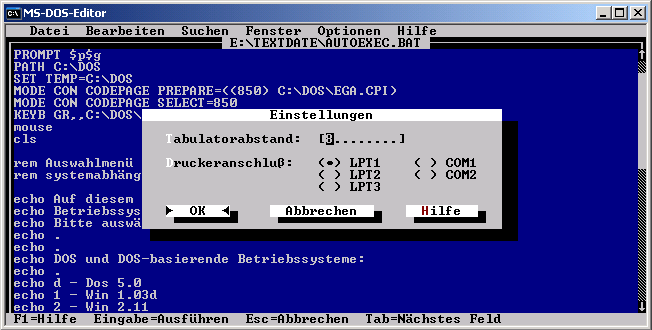
\includegraphics[scale=0.8]{imagens/EDIT_MSDOS.png}
    \\\textbf{Fonte: Internet Archive} \label{fig:EDIT_MSDOS}
\end{figure}
\FloatBarrier

Mais adiante na história, com o avanço das interfaces gráficas os editores de
texto passaram a se tornar mais visuais. É possível notar essa evolução em \textit{softwares}
como o Notepad++ \cite{NotepadPlusPlus2025} até editores mais famosos como
Visual Studio Code \cite{VSCode2025} e o recente Zed \cite{ZedEditor2025}. Esses
editores de texto modernos oferecem uma ampla gama de recursos, como
customização e extensibilidade, suporte a plugins, integração com sistemas de
controle de versão, destacamento de sintaxe, autocompletar, entre outros,
tornando a edição de texto mais eficiente e produtiva.

O Notepad++ é um editor de texto de código aberto que se destaca por sua leveza
e simplicidade, oferecendo uma interface amigável e recursos avançados para edição
de código-fonte. Ele suporta várias linguagens de programação e possui recursos
como realceamento de sintaxe, autocompletar, busca avançada e suporte a \textit{plugins},
tornando-o uma escolha popular entre usuários que buscam um editor de texto
simples mas eficiente.

Por outro lado o Visual Studio Code é um editor de código-fonte desenvolvido
pela Microsoft que se tornou extremamente popular devido à sua extensibilidade e
integração com diversas ferramentas de desenvolvimento, além de oferecer uma ampla
gama de recursos como depuração integrada, controle de versão, suporte a várias linguagens
de programação e uma vasta biblioteca de extensões, permitindo que os usuários
personalizem sua experiência de edição de texto de acordo com suas necessidades.

\FloatBarrier
\begin{figure}[!htbp]
    \centering
    \caption{Visual Studio Code}
    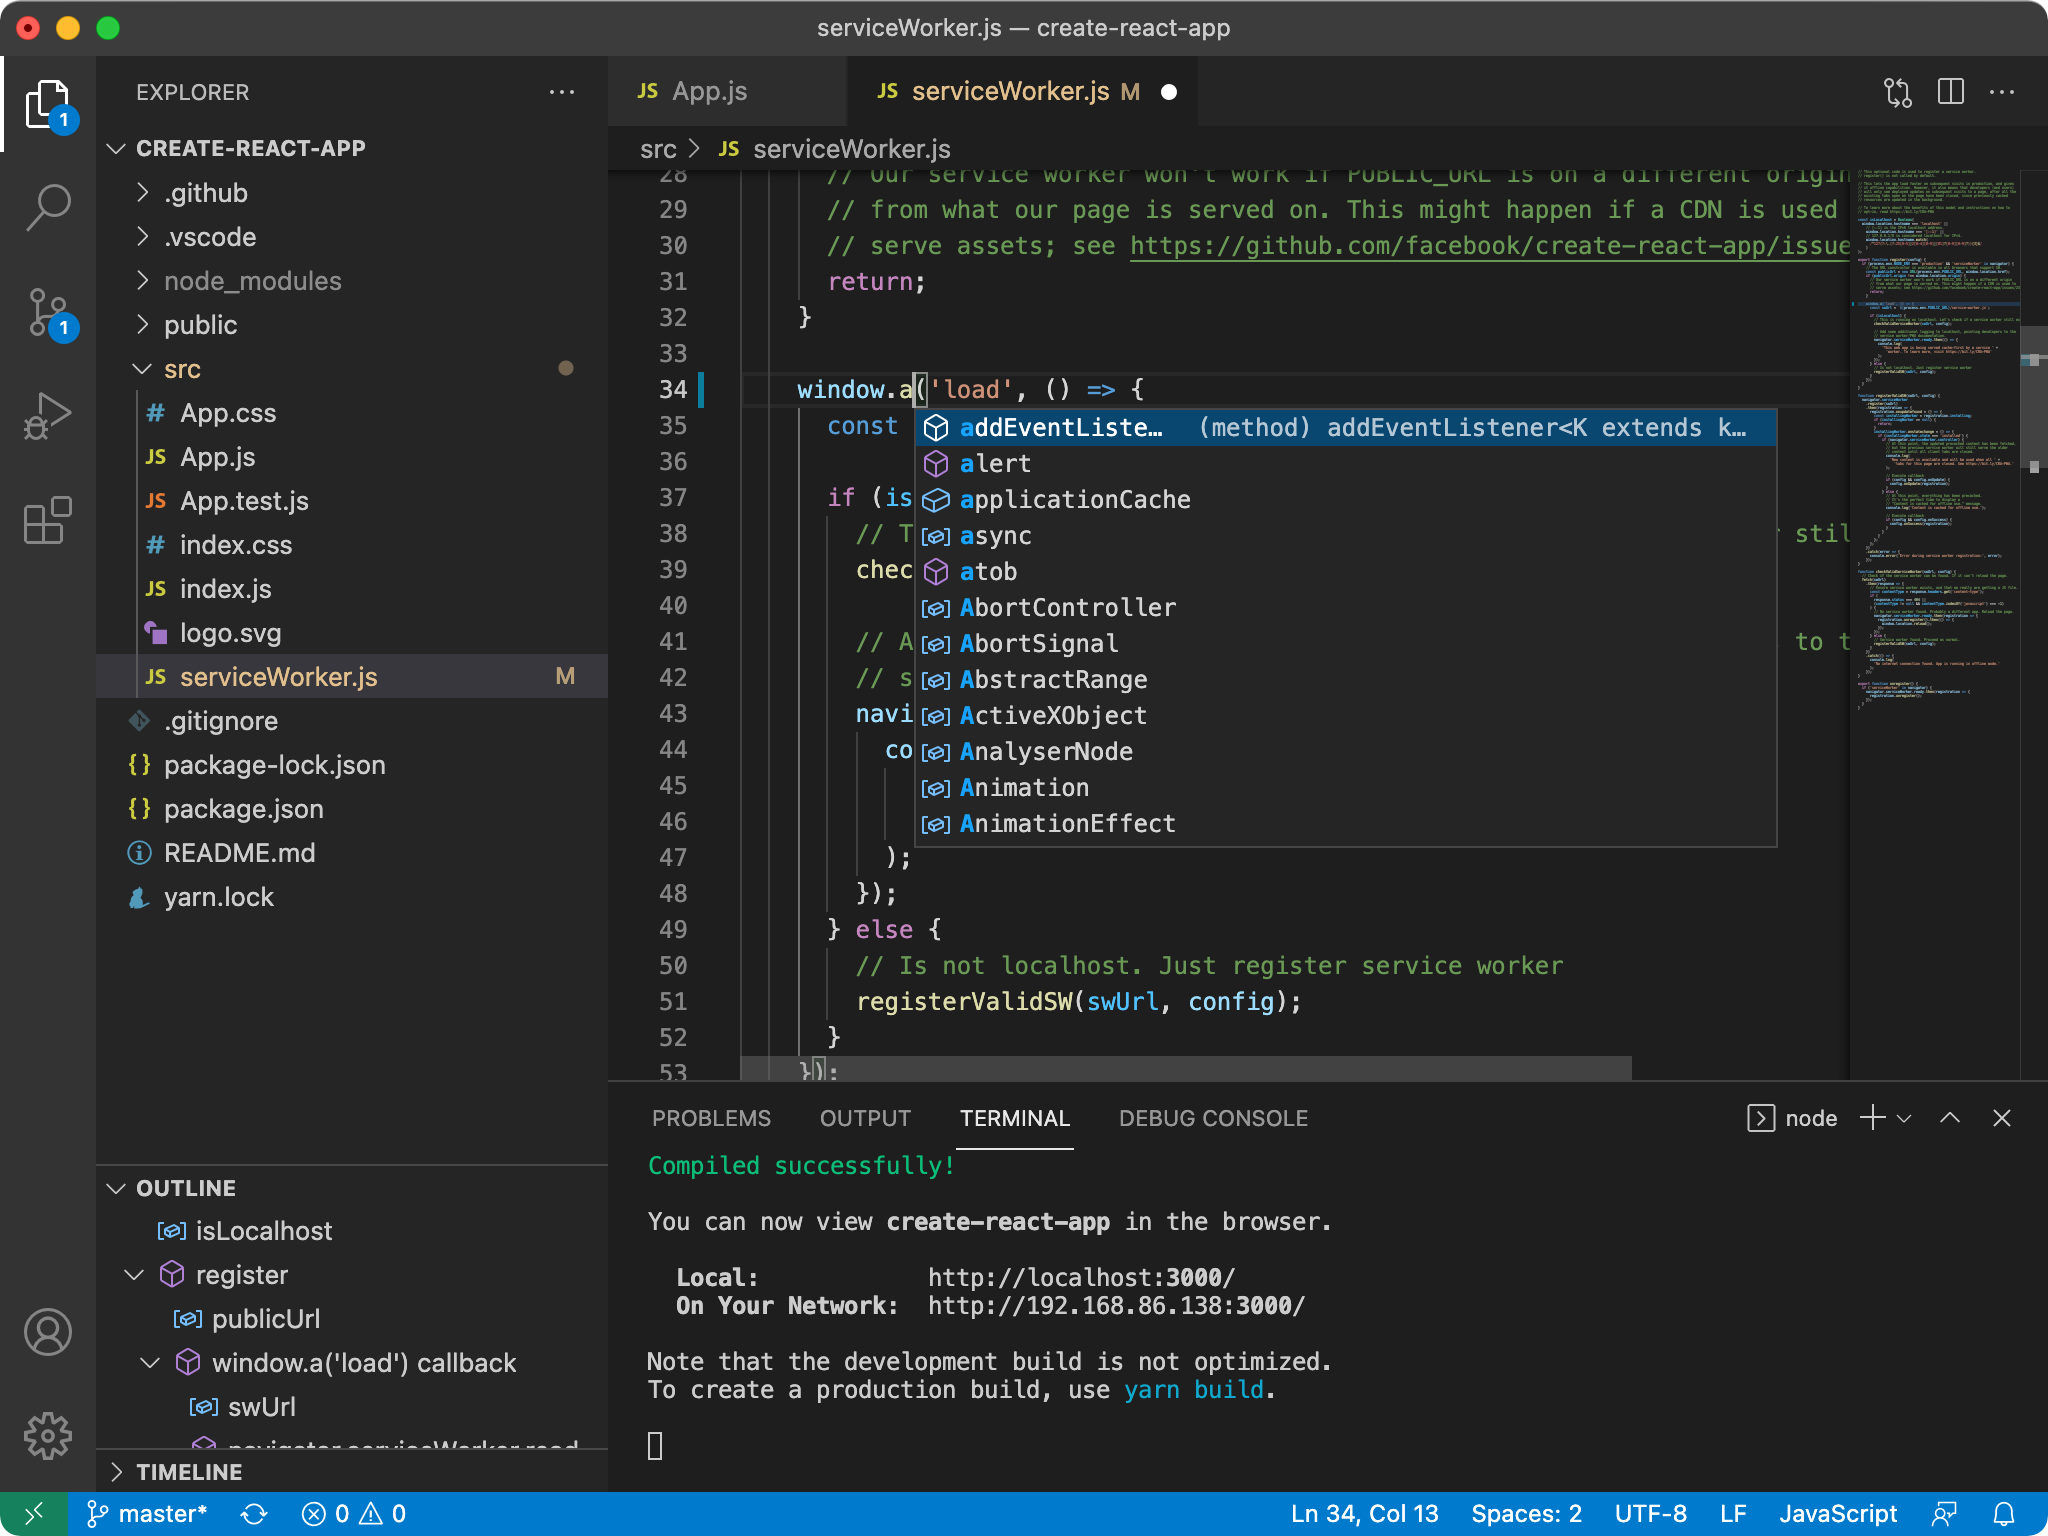
\includegraphics[scale=0.3]{imagens/VSCode.png}
    \\\textbf{Fonte: Github Microsoft - Visual Studio Code} \label{fig:VSCode}
\end{figure}
\FloatBarrier

Já o ainda em desenvolvimento Zed Editor se destaca por sua abordagem colaborativa
e em tempo real, permitindo que vários usuários editem o mesmo arquivo
simultaneamente. Ele oferece uma interface moderna e intuitiva e que se assemelha
muito ao Visual Studio Code, com recursos como realceamento de sintaxe, autocompletar,
integração com sistemas de controle de versão e suporte a \textit{plugins},
tornando-o uma escolha interessante para equipes de desenvolvimento que buscam
uma experiência de edição colaborativa e eficiente.

De modo geral, as interfaces podem ser divididas em dois grandes grupos: CLI e
GUI. Como apontados, as CLIs exigem um conhecimento técnico mais avançado, já que
utilizam constantemente de atalhos de teclado (ou do inglês, \textit{shortcuts}),
gerando uma curva de aprendizado mais íngreme, porém, com poder de controle
maior e fluidez na utilização diária, já que são interfaces altamente customizáveis
e cada usuário pode ter seu \textit{setup}. Por sua vez, as GUIs são mais
intuitivas por oferecerem elementos visuais como menus e ícones, facilitando o uso
e oferecendo experiência \textit{plug-and-play} (experiência de uso imediato), e
popularizando o computador como ferramenta pessoal.

Ainda hoje, após décadas de evolução, há usuários que preferem interagir por meio
de CLIs, como ao utilizar o editor NeoVim em sistemas UNIX. Com base nisso, este
trabalho propõe a criação de um editor CLI com uma interface mais moderna e
intuitiva, buscando unir o poder e a eficiência das CLIs à facilidade de uso presente
nas GUIs.

\section{Manipulação e Edição de Texto}

Portanto, no campo da computação, a existência de ferramentas que lidam com a
manipulação e escrita de programas é, sem dúvidas, essencial. Mas o mundo da edição
de texto é vasto e diversificado, abrangendo desde simples e comuns editores de
texto usados diariamente até sofisticados e completos ambientes de
desenvolvimento.

\subsection{Processadores de Texto}

Um processador de texto é qualquer \textit{software} comummente utilizado para a
criação, edição ou formatação e exportação de textos digitais. Esses programas
oferecem uma ampla gama de ferramentas e funcionalidades que facilitam o dia a
dia de quem lida com documentos, seja para fins pessoais, acadêmicos ou
profissionais.

O Microsoft Word\footnote{Disponível em: https://www.microsoft.com/en-us/microsoft-365/word}
foi um marco na história dos processadores de texto nos anos 80, já que, entre seus
diversos concorrentes, trouxe um novo paradigma de escrita: da máquina de escrever
ao computador \cite{inbook}. Atualmente, o ainda consolidado Word oferece uma vasta
gama de recursos, como verificação ortográfica e gramatical, formatação avançada,
inserção de imagens e tabelas, além de suporte a diversos formatos de arquivo.

Outro exemplo de processador de texto é o LibreOffice Writer\footnote{Disponível
em: https://www.libreoffice.org/}, parte do conjunto de aplicativos LibreOffice,
que é uma alternativa de código aberto ao Microsoft Word. Também merece destaque
o Google Documents\footnote{Disponível em: https://docs.google.com/}, uma ferramenta
baseada na nuvem que permite a criação e edição de documentos em tempo real,
ideal para colaboração.

Mas a sua estrutura vai muito além. Tais ferramentas são projetadas usando \textit{buffers}
de texto. Pense nisso: quando o usuário digita um caractere ele é inserido em um
\textbf{\textit{buffer} de edição}, uma estrutura em memória que mantém o
conteúdo do documento em tempo real, permitindo manipulações rápidas, como
inserções, remoções e formatações, sem acessar diretamente o arquivo no disco. Somente
quando o usuário salva o documento (ou ocorre um salvamento automático) é que o conteúdo
de fato é gravado permanentemente no arquivo de armazenamento \cite{Jacobson1989}.

\subsection{Editores}

Avançando, outras alternativas (e as mais comuns para pessoas da área) são os editores
de texto voltados a programação. Esses editores são especificamente projetados
para lidar com código-fonte de linguagem de programação, e oferece uma vasta gama
de recursos, como os citados anteriormente.

Dentro desse grupo foi visto dois grandes subgrupos: GUI e CLI. A CLI foca em "interfaces"
de linha de comando, sendo editores de \textit{shell} (ou terminais) como o Vi/Vim/NeoVim
e Emacs e seus derivados. Ainda podemos ter editores CLI mais simples, porém
funcionais, como Nano e EDIT. A GUI por sua vez foca em interfaces gráficas, como
o Notepad++, Visual Studio Code e Zed.

A forma como esses editores funcionam é similar aos processadores de texto, com singelas
diferenças na forma de lidar com o conteúdo. Eles também utilizam \textit{buffers}
de texto para manter o conteúdo do documento em memória, no entanto, como esses editores
são voltados para programação, funcionalidades já descritas antes como
realceamento de sintaxe, autocompletar e entre outros estão presentes. Além
disso, esses editores frequentemente suportam múltiplos \textit{buffers} ou abas,
permitindo que os desenvolvedores trabalhem em vários arquivos simultaneamente.

Aqui, podemos seguir alguns principios de funcionamento dos \textit{buffers}:

\begin{itemize}
    \item Evento de tecla -> fila de eventos;

    \item Buffer de edição (RAM) -> o editor aplica a operação (inserir/apagar)
        em uma estrutura interna que representa o documento;

    \item Histórico/\textit{undo} -> a operação é registrada (por \textit{log} de
        comandos, \textit{snapshots} ou ambos);

    \item Tela -> um \textit{buffer} de renderização recalcula apenas o que mudou
        (linha, trecho, \textit{layout});

    \item Persistência -> só vai ao disco quando você manda salvar (ou quando o auto-save
        dispara). Antes disso, a maior parte está em memória, mas mesmo ao salvar,
        bibliotecas padrão e o SO aplicam \textit{line/full buffering} antes de gravar
        no arquivo físico;
\end{itemize}
\cite{glibc-buffering-concepts}.

\subsection{IDEs}

Cabe aqui ressaltar os ambientes de desenvolvimento integrados (IDEs), que são ferramentas
mais completas que os editores de texto, trazendo outras funcionalidades
essenciais. Essas ferramentas oferecem recursos que auxiliam o ciclo de vida de desenvolvimento,
e geralmente possuem seu próprio editor de texto embutido, com compilador/depurador
integrado, ferramentas de build e automação, perfis de projeto, entre outras
funcionalidades.

As IDEs normalmente são projetadas para suportar uma única linguagem de
programação, como o CodeBlocks \cite{codeblocks}, voltadas para a fámilia C (C++
e C); ou as ferramentas da JetBrains \cite{jetbrains_tools} (IntelliJ IDEA, PyCharm,
etc.), voltadas para Java e Python, respectivamente. Outras IDEs, como o Visual
Studio \cite{visual_studio} suporta várias linguagens, igualmente o Eclipse \cite{eclipse_ide}
e o NetBeans \cite{netbeans_ide}, mas com foco em um ecossistema específico, como
o desenvolvimento Java.

\FloatBarrier
\begin{figure}[!htbp]
    \centering
    \caption{Visual Studio 2022}
    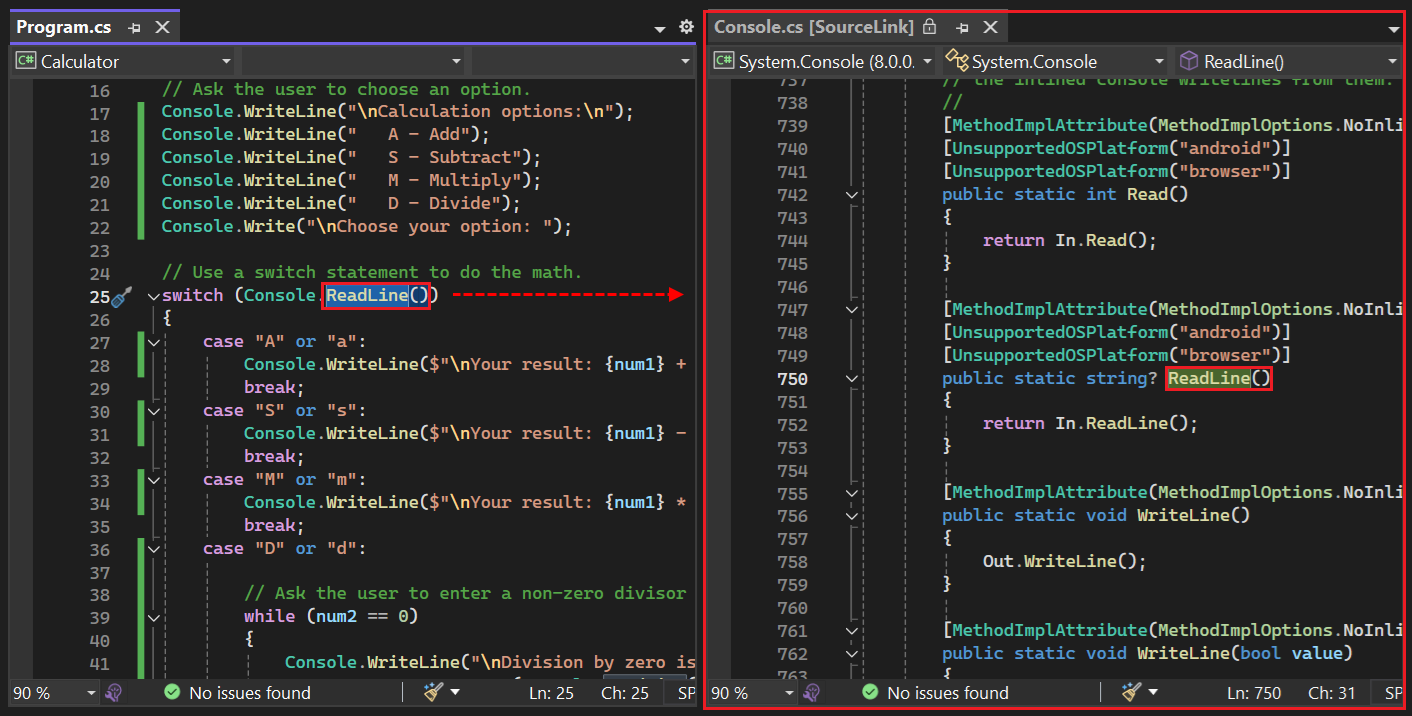
\includegraphics[scale=0.4]{imagens/VisualStudio.png}
    \\\textbf{Fonte: Microsoft - Visual Studio} \label{fig:VisualStudio}
\end{figure}
\FloatBarrier

Vale destacar que o Visual Studio Code, apesar de ser um editor de texto, é
frequentemente utilizado como uma "IDE" graças à sua extensibilidade e
integração com diversas ferramentas, podendo ser chamado de "canivete suíço" para
os desenvolvedores.

\section{Principais Bibliotecas para Controle de Terminal em Linguagem C}

Diversas linguagens de programação, como Go, Python\footnote{Linguagem de
programação. Disponível em: https://www.python.org/}, Rust\footnote{Linguagem de
programação. Disponível em: https://www.rust-lang.org/pt-BR} e Java\footnote{Linguagem
de programação. Disponível em: https://www.java.com/pt-BR/}, oferecem suporte ao
desenvolvimento de aplicações em interfaces de linha de comando. Nesta seção, são
apresentadas as principais bibliotecas utilizadas para o controle de terminais em
linguagem C. A escolha dessa linguagem para o desenvolvimento do NITE justifica-se
por sua flexibilidade e alto desempenho.

\subsection{NCURSES e CURSES}

A biblioteca Curses foi desenvolvida por Ken Arnold em 1978, e fornece um
conjunto de funções para manipulação de telas em modo texto. O nome "Curses" é um
trocadilho para "\textit{cursor optimization}", já que a biblioteca foi projetada
para otimizar o uso do cursor em terminais de texto. Podemos delimitar alguns
conceitos importantes para Curses, onde a tela do terminal é manipulada por meio
de estruturas chamadas \textit{windows} (janelas), que funcionam como arranjos bidimensionais
representando parte ou toda a exibição. Existem janelas padrão, como a \textbf{stdscr}
(tela inteira) e o \textbf{curscr} (estado atual da tela, não modificável). Cada
janela mantém a posição de um cursor lógico, enquanto o cursor físico é único e
aparece de fato na tela. Além disso, o curses permite criar \textit{pads},
janelas que não se limitam ao tamanho da tela. \cite{ibm_curses_aix}

Já a Ncurses é um clone da Curses, com suas melhorias. Teve inicio por volta de
1982 com Pavel Curtis com o nome de Pcurses, e a partir de 86, várias pessoas
começaram a contribuir com o projeto. A \textit{New Curses} (Ncurses) em 1993
foi aprimorada e passou a ser mantida por Zeyd Ben-Halim, recebendo algumas correções
de bugs e até reformatação. Eric S. Raymond assumiu a manutenção em 1996, e em
1998, Thomas E. Dickey começou a contribuir com o projeto, tornando-se o mantenedor
principal em 2001, cargo que ocupa até hoje. Juergen Pfeifer também contribuiu significativamente
para o projeto adicionando bibliotecas \textbf{\textit{forms} e menus}, e Warren
Tucker adicionou a biblioteca \textbf{\textit{panel}}. \cite{ncurses_site}

\vspace{0.4cm}
\lstinputlisting[language=c]{fontes/NcursesExemplo.c}
\vspace{0.4cm}

Mas o que exatamente a Ncurses oferece? Ela fornece funções para mover o cursor,
criar janelas, produzir cores, interagir com o mouse etc. Assim, os programas não
precisam se preocupar com as capacidades específicas do terminal subjacente.
Sendo totalmente compatível com as versões anteriores da Curses, não apenas cria
uma camada sobre as capacidades do terminal, mas também fornece uma estrutura
robusta para criar interfaces em modo texto (TUI). Com suas bibliotecas associadas
(\textit{panel}, menu e \textit{form}) é possível criar aplicações que contenham
múltiplas janelas, menus, painéis e formulários de maneira simples e eficiente
\cite{ncurses_howto}.

\FloatBarrier
\begin{figure}[!htbp]
    \centering
    \caption{Protótipo do NITE em execução no terminal utilizando Ncurses}
    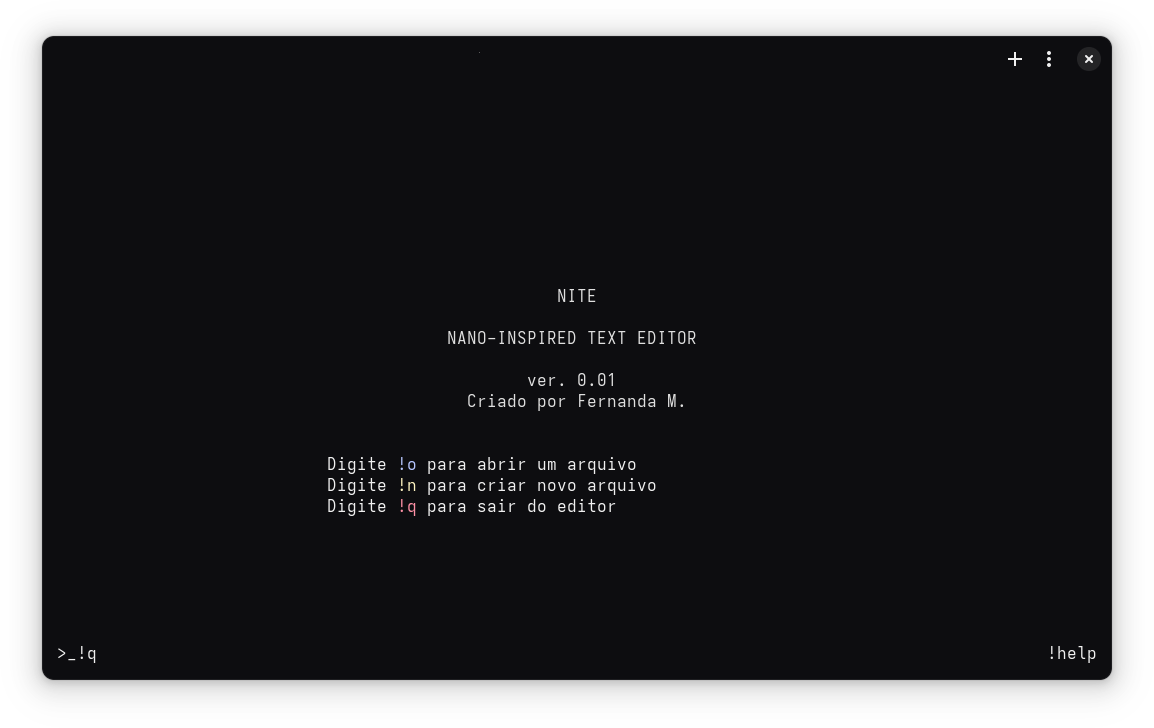
\includegraphics[scale=0.3]{imagens/NITE.png}
\end{figure}
\FloatBarrier

A biblioteca ncurses foi escolhida como principal ferramenta para o desenvolvimento
do NITE devido à sua maturidade, estabilidade e ampla utilização na comunidade. Além
disso, é considerada o padrão para a criação de editores de terminal complexos, embora
apresente uma curva de aprendizado mais acentuada.

\subsection{TERMBOX e TERMBOX2}

Mas não apenas de bibliotecas complexas a linguagem C vive. Existem também bibliotecas
mais simples, e esse é o objetivo da Termbox. Desenvolvida em 2010\footnote{Disponível
em: https://github.com/termbox/termbox}, a ideia da mesma é, além de simples, ser
eficiente e portátil.

A Terbox tem como ideia uma abstração simples ao enxergar o terminal como uma grade
de células fixas com fluxo de mensagens estruturadas e foi inspirada na API\footnote{Sigla
para Application Programming Interface, é um conjunto de regras e ferramentas que
permite que diferentes softwares “conversem” entre si, definindo como um
programa pode usar funcionalidades de outros sem precisar conhecer todos os
detalhes internos de como ele foi implementado.} de console do Windows. Mas a execução
não é perfeita, visto que caracteres mais largos (como caracteres do alfabeto chines,
japonês ou coreano) não são compatíveis com a ideia de uma TUI simples \cite{termbox_googlecode}.

\vspace{0.4cm}
\lstinputlisting[language=c]{fontes/TermboxExemplo.c}
\vspace{0.4cm}

Sendo descontinuada em 2020, o projeto da Termbox2\footnote{Disponível em: https://github.com/termbox/termbox2}
se iniciou em 2021 e é um \textit{fork}\footnote{"Bifurcação"; O projeto original
é copiado e modificado livremente} da Termbox original que visa corrigir bugs e
adicionar novos recursos, mantendo a simplicidade e eficiência da biblioteca padrão.
Também busca ser uma alternativa direta a Ncurses, com uma API mais fácil de se usar
e entender \cite{termbox2_github}.

\vspace{0.4cm}
\lstinputlisting[language=c]{fontes/Termbox2Exemplo.c}
\vspace{0.4cm}

\subsection{TERMCAP e TERMINFO}

Já o Termcap é uma biblioteca e banco de dados mais antigo, que fornece uma
interface para acessar as capacidades dos terminais de texto. Desenvolvido pelo criador
do Vi, Bill Joy, o Termcap foi amplamente utilizado em sistemas UNIX durante os anos
80 e 90, principalmente após a implementação do Termcap por Richard M. Stallman,
criador do Emacs.

Segundo a documentação do GNU Termcap \cite{stallman_termcap}, a biblioteca foi desenvolvida
para permitir que programas realizem saída de caracteres sem depender diretamente
das particularidades de cada terminal. Os programas podem ler o Termcap para
encontrar os códigos de escape (ANSI) específicos cujo são necessários para
controlar o terminal \cite{kerrisk_termcap_man7}.

\vspace{0.4cm}
\lstinputlisting[language=c]{fontes/TermcapExemplo.c}
\vspace{0.4cm}

Atualmente é mantido apenas por questões de compatibilidade, já que o Terminfo é
a alternativa mais moderna e flexível. O Terminfo segue a mesma linha do Termcap,
mas com um banco de dados mais estruturado e eficiente em terminais que possam
não utilizar as Curses. Ele foi desenvolvido para superar as limitações do Termcap
e especifica quais sequências de escape ou caracteres de controle devem ser enviadas
ao terminal para realização de tarefas específicas, como mover o cursor, limpar a
tela ou alterar cores. O Terminfo também é mais simples de se usar, com uma API mais
direta e fácil de entender. \cite{man7_terminfo, tldp_text_terminal_howto}

\vspace{0.4cm}
\lstinputlisting[language=c]{fontes/TerminfoExemplo.c}
\vspace{0.4cm}

\subsection{S-LANG}

Voltando para as bibliotecas mais completas, a S-Lang é uma biblioteca de
programação que oferece uma ampla gama de funcionalidades, permitindo a criaçao de
\textit{softwares} multiplataformas de forma robusta. O recurso mais interessante
é seu interpletador, que pode facilmente tornar um programa extensível e suporta
todos os tipos de inteiros da linguagem C (\textit{char, short, int, long e long
long}), além de um suporte notável ao usar estruturas como \textit{arrays}.

A biblioteca possui ferramentas para recursos como gerenciamento de tela, mapa
para teclas, entrada/saída de terminal, entre outros. A S-Lang também possui aplicativo
independente chamado \textbf{slsh} (S-lang \textit{shell}), que pode ser usado
em aplicações baseadas na S-Lang, podendo acessar de forma iterativa todos os componentes
de seu interpletador \cite{Davis2022S_Lang}.

\vspace{0.4cm}
\lstinputlisting[language=c]{fontes/SlangExemplo.c}
\vspace{0.4cm}